\documentclass{article}

\usepackage{graphicx}
\usepackage{tikz}
\usepackage{tikzsymbols}
\usetikzlibrary{calc,patterns,shapes.geometric}
\pagestyle{empty}
\usepackage[margin=0pt]{geometry}
\geometry{papersize={14in,12in}}

\def\centerarc[#1](#2)(#3:#4:#5){\draw[#1] ($(#2)+({#5*cos(#3)},{#5*sin(#3)})$) arc (#3:#4:#5);}

\begin{document}
	\begin{figure}
		\centering
		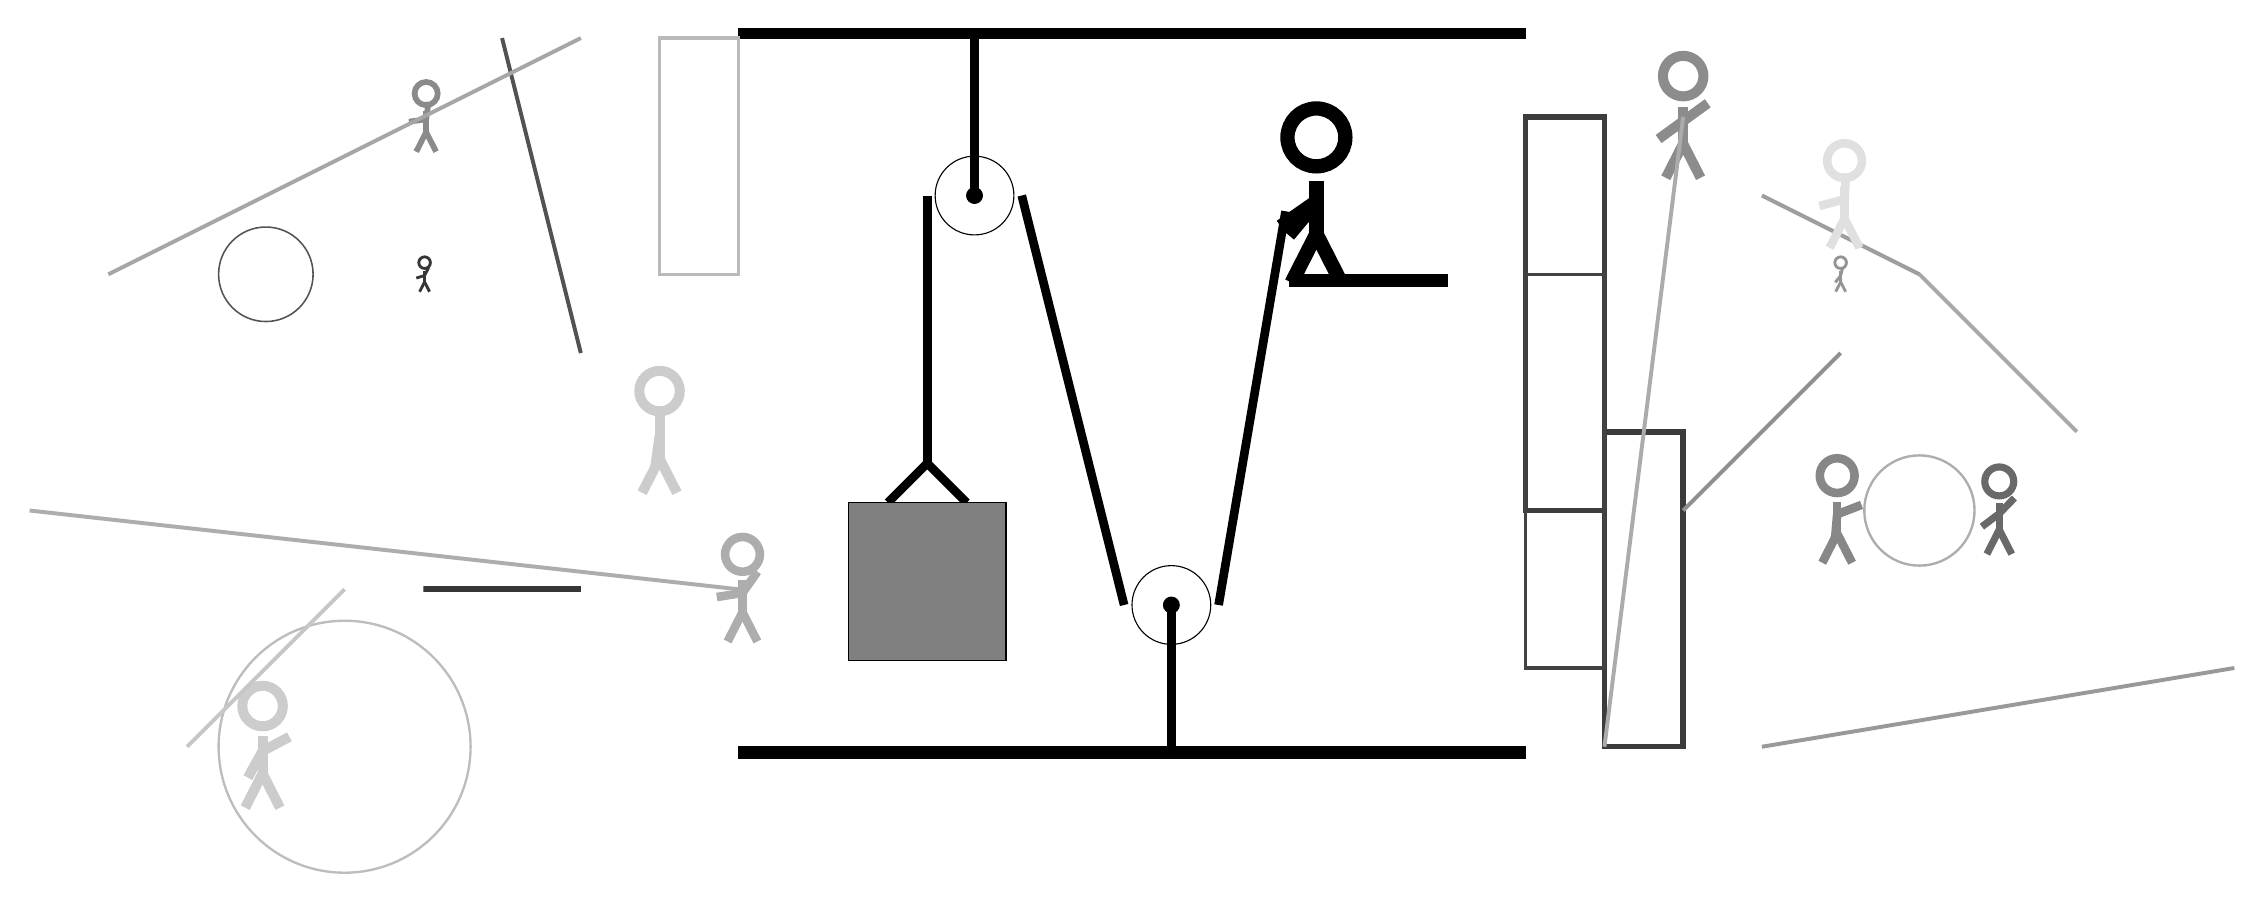
\begin{tikzpicture}
			%%%%% START %%%%%
			
			\draw[fill=black] (-2, 9) rectangle (8, 9.125);
			
			\node[line width=0.3mm, color=black!59] at (14, 3) {\Strichmaxerl[5][37][46]};
			
			\node[line width=0.5mm, color=black!46] at (-6, 8) {\Strichmaxerl[4][8][82]};
			\node[line width=0.5mm, color=black!20] at (-8, 0) {\Strichmaxerl[7][61][28]};
			\draw[line width=0.7mm, color=black!77] (9, 0) rectangle (10, 4);
			\draw [line width=0.3mm, color=black!32](13, 3) circle (0.7);
			
			\node[line width=0.5mm, color=black!20] at (-3, 4) {\Strichmaxerl[7][82][90]};
			\draw[line width=0.7mm, color=black!79] (-4, 2) rectangle (-6, 2);
			
			\node[line width=0.7mm, color=black!79] at (-6, 6) {\Strichmaxerl[2][17][63]};
			\draw[line width=0.5mm, color=black!32](-2, 2) -- (-11, 3);
			
			\draw[line width=0.5mm, color=black!34](13, 6) -- (15, 4);
			
			\draw[line width=0.7mm, color=black!76] (9, 3) rectangle (8, 8);
			
			\node[line width=0.3mm, color=black!45] at (10, 8) {\Strichmaxerl[7][36][36]};
			\draw [line width=0.3mm, color=black!26](-7, 0) circle (1.6);
			\node[line width=0.7mm, color=black!47] at (12, 3) {\Strichmaxerl[6][85][21]};
			\node[line width=0.2mm, color=black!32] at (-2, 2) {\Strichmaxerl[6][9][55]};
			\draw[line width=0.5mm, color=black!68](-4, 5) -- (-5, 9);
			\draw[line width=0.4mm, color=black!74] (9, 1) rectangle (8, 6);
			\draw [line width=0.2mm, color=black!67](-8, 6) circle (0.6);
			\draw[line width=0.5mm, color=black!35](-4, 9) -- (-10, 6);
			\draw[line width=0.5mm, color=black!33](9, 0) -- (10, 8);
			\draw[line width=0.4mm, color=black!27] (-3, 6) rectangle (-2, 9);
			\draw[line width=0.5mm, color=black!38](11, 7) -- (13, 6);
			
			\draw[line width=0.5mm, color=black!44](12, 5) -- (10, 3);
			\draw[line width=0.5mm, color=black!22](-7, 2) -- (-9, 0);
			\draw[line width=0.5mm, color=black!40](11, 0) -- (17, 1);
			\node[line width=0.7mm, color=black!12] at (12, 7) {\Strichmaxerl[6][15][87]};
			\node[line width=0.2mm, color=black!42] at (12, 6) {\Strichmaxerl[2][52][75]};
			
			\draw (3.5, 1.8) circle (0.5);
			\draw[fill=black] (3.5, 1.8) circle (0.1);
			\draw[line width=1.1mm] (3.5, 1.8) -- (3.5, 0);
			
			\draw (1, 7) circle (0.5);
			\draw[fill=black] (1, 7) circle (0.1);
			\draw[line width=1.1mm] (1, 9) -- (1, 7);
			
			\draw[line width=1.1mm](-0.1, 3.1) --  (0.4, 3.6) -- (0.9, 3.1);
			\draw[fill=black!50] (-0.6, 3.1) rectangle (1.4, 1.1);
			
			\draw[line width=1.1mm](0.4, 7) -- (0.4, 3.6);
			\centerarc[line width=1.1mm](1, 7)(180:0:0.6)
			\draw[line width=1.1mm](1.6, 7) -- (2.9, 1.8);
			\centerarc[line width=1.1mm](3.5, 1.8)(180:360:0.6)
			\draw[line width=1.1mm](4.1, 1.8) -- (4.95, 6.8);
			
			\node at (5.3, 7) {\Strichmaxerl[10][35][-130]};
			\draw[fill=black] (5, 6) rectangle (7, 5.85);
			
			\draw[fill=black] (-2, 0) rectangle (8, -0.15);
			
			%%%%% END %%%%%
		\end{tikzpicture}
	\end{figure}	
\end{document}